\documentclass[a4paper,14pt]{extreport} % формат документа

\usepackage{amsmath}
\usepackage{cmap} % поиск в ПДФ
\usepackage[T2A]{fontenc} % кодировка
\usepackage[utf8]{inputenc} % кодировка исходного текста
\usepackage[english,russian]{babel} % локализация и переносы
\usepackage[left = 1.5cm, right = 1cm, top = 2cm, bottom = 2 cm]{geometry} % поля
\usepackage{listings}
\usepackage{graphicx} % для вставки рисунков
\usepackage{amsmath}
\usepackage{float}
\usepackage{multirow}
\usepackage{longtable}
\usepackage{array}
\graphicspath{{img/}}
\DeclareGraphicsExtensions{.pdf,.png,.jpg}
\newcommand{\anonsection}[1]{\section*{#1}\addcontentsline{toc}{section}{#1}}

\lstset{ %
	language=Lisp,                % Язык программирования 
	numbers=left,                   % С какой стороны нумеровать          
	frame=single,                    % Добавить рамку
}

\begin{document}
\begin{titlepage}

    \begin{table}[H]
        \centering
        \footnotesize
        \begin{tabular}{cc}
            \multirow{8}{*}{
\includegraphics[scale=0.35]{bmstu.jpg}}
            & \\
            & \\
            & \textbf{Министерство науки и высшего образования Российской Федерации} \\
            & \textbf{Федеральное государственное бюджетное образовательное учреждение} \\
            & \textbf{высшего образования} \\
            & \textbf{<<Московский государственный технический} \\
            & \textbf{университет имени Н.Э. Баумана>>} \\
            & \textbf{(МГТУ им. Н.Э. Баумана)} \\
        \end{tabular}
    \end{table}

    \vspace{-2.5cm}

    \begin{flushleft}
        \rule[-1cm]{\textwidth}{3pt}
        \rule{\textwidth}{1pt}
    \end{flushleft}

    \begin{flushleft}
        \small
        ФАКУЛЬТЕТ
        \underline{<<Информатика и системы управления>>\ \ \ \ \ \ \ 
        \ \ \ \ \ \ \ \ \ \ \ \ \ \ \ \ \ \ \ \ \ \ \ \ \ \ \ \ \ \ \ 
    \ \ \ \ \ \ \ \ \ \ \ \ \ \ \ } \\
        КАФЕДРА
        \underline{<<Программное обеспечение ЭВМ и
        информационные технологии>>
        \ \ \ \ \ \ \ \ \ \ \ \ \ \ \ \ \ \ \ \ }
    \end{flushleft}

    \vspace{2cm}

    \begin{center}
        \textbf{Лабораторная работа № 6} \\
        \vspace{0.5cm}
    \end{center}

    \vspace{4cm}

    \begin{flushleft}
        \begin{tabular}{ll}
            \textbf{Дисциплина} & Компьютерные сети.  \\
            \textbf{Тема} & Разбиение сети на подсети. \\
            & Настройка DHCP-сервера в сетевом эмуляторе.  \\
            \\
            \textbf{Студент} & Сиденко А.Г. \\
            \textbf{Группа} & ИУ7-73Б \\
            \textbf{Вариант} & 18\\
            \textbf{Преподаватель} & Рогозин Н.О.  \\
        \end{tabular}
    \end{flushleft}

    \vspace{4cm}

   \begin{center}
        Москва, 2020 г.
    \end{center}

\end{titlepage}

Для локальной общей сети был выделен частный адрес \textbf{127.168.18.0/24}. 

\begin{enumerate}

\item Разделить сеть на 5 подсетей

\begin{longtable}{|m{0.8cm}|m{1.3cm}|m{2.6cm}|m{2.6cm}|m{2.6cm}|m{2.6cm}|m{3.1cm}|}
\hline
Но- мер сети & Число хостов в подсети & Номер подсети & Первый IP & Последний IP & Широкове- щательный адрес  & Маска  \\ \hline
1 &28 & 192.168.18.0 & 192.168.18.1 & 192.168.18.30 & 192.168.18.31  & 255.255.255.224 (27)  \\ \hline
2 &5 & 192.168.18.64 & 192.168.18.65 & 192.168.18.70 & 192.168.18.71  & 255.255.255.248 (29)  \\ \hline
3 &2 & 192.168.18.80 & 192.168.18.81 & 192.168.18.82 & 192.168.18.83  & 255.255.255.252 (30)  \\ \hline
4 &5 & 192.168.18.72 & 192.168.18.73 & 192.168.18.78 & 192.168.18.79  & 255.255.255.248 (29)  \\ \hline
5 &28 & 192.168.18.32 & 192.168.18.33 & 192.168.18.62 & 192.168.18.63  & 255.255.255.224 (27)  \\ \hline
\caption{Разбинение сети на подсети. }
\label{table:1}
\end{longtable}

Число хостов в подсети -- это необходимое число хостов, заданное в условии. 

Для получение подсетей разного размера, вначале выделялись наибольшие, затем свободные наибольшие делились на подсети меньшего размера.

\newpage 

\item Настройка отдельного DHCP-сервера для 1 подсети

\begin{figure}[H]
  \centering
  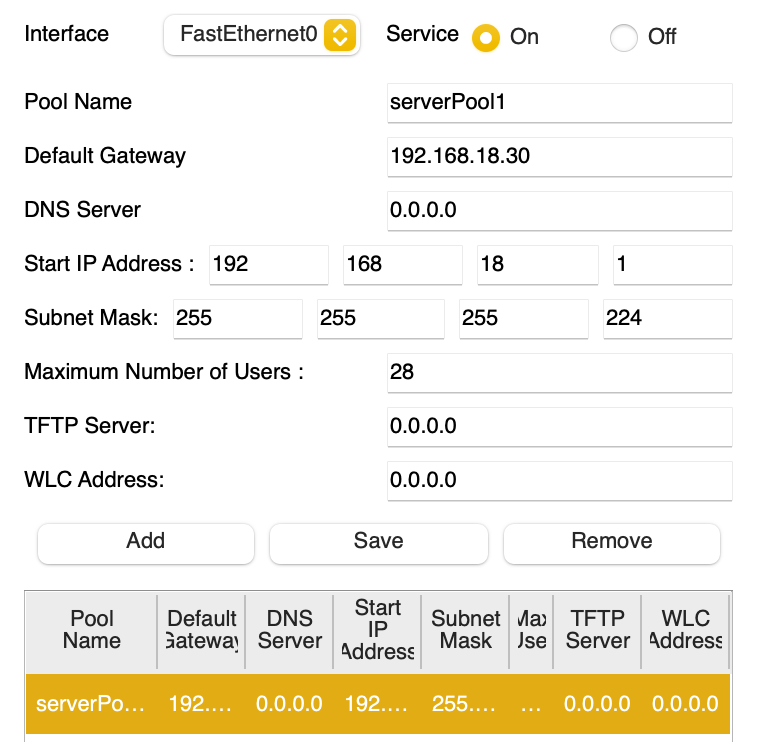
\includegraphics[scale=0.7]{1}
  \caption{Настройка сервера. }
\end{figure}

\begin{figure}[H]
  \centering
  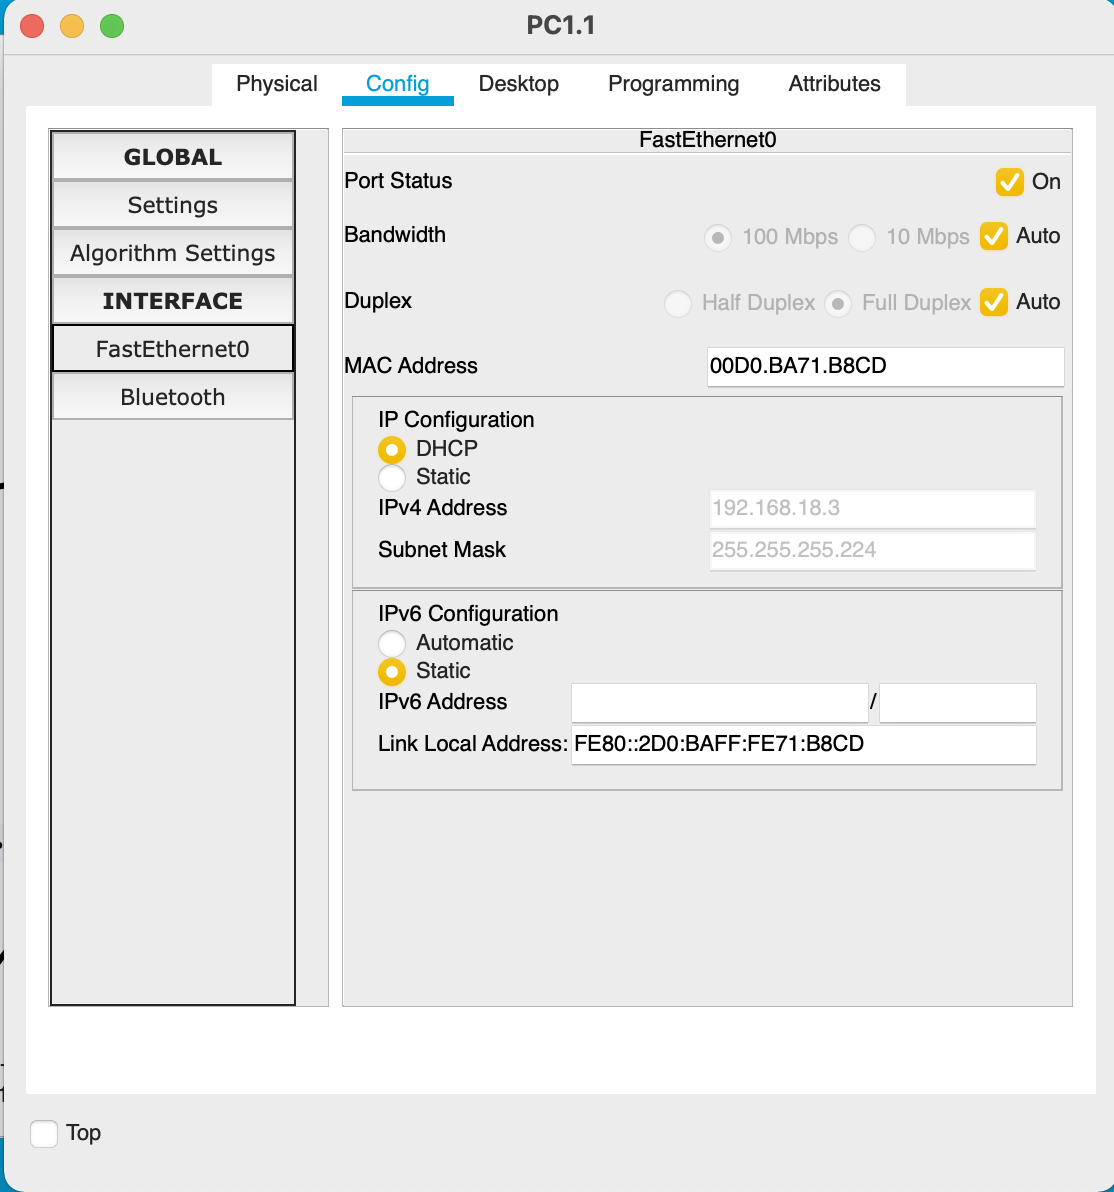
\includegraphics[scale=0.6]{2}
  \caption{Проверка автоматически установленного адреса хоста. }
\end{figure}

\item Настроить в качестве DHCP-сервера маршрутизаторы для подсетей 2,4,5. 

\begin{figure}[H]\center
	\begin{tabular}{cc}
		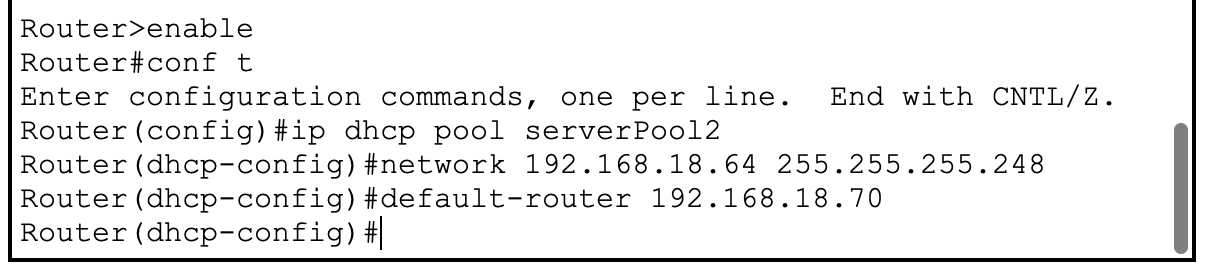
\includegraphics[scale=0.7]{3}\\
		 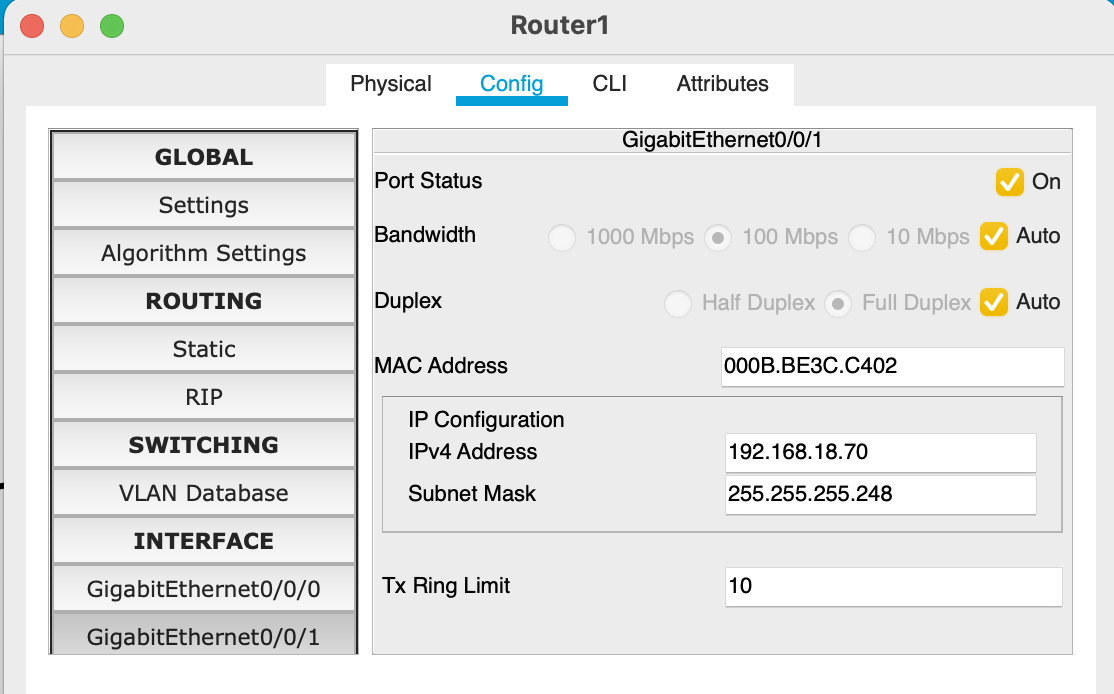
\includegraphics[scale=0.7]{4} \\
	\end{tabular}
	\caption{Настройка сервера. }
\end{figure}

\begin{figure}[H]
  \centering
  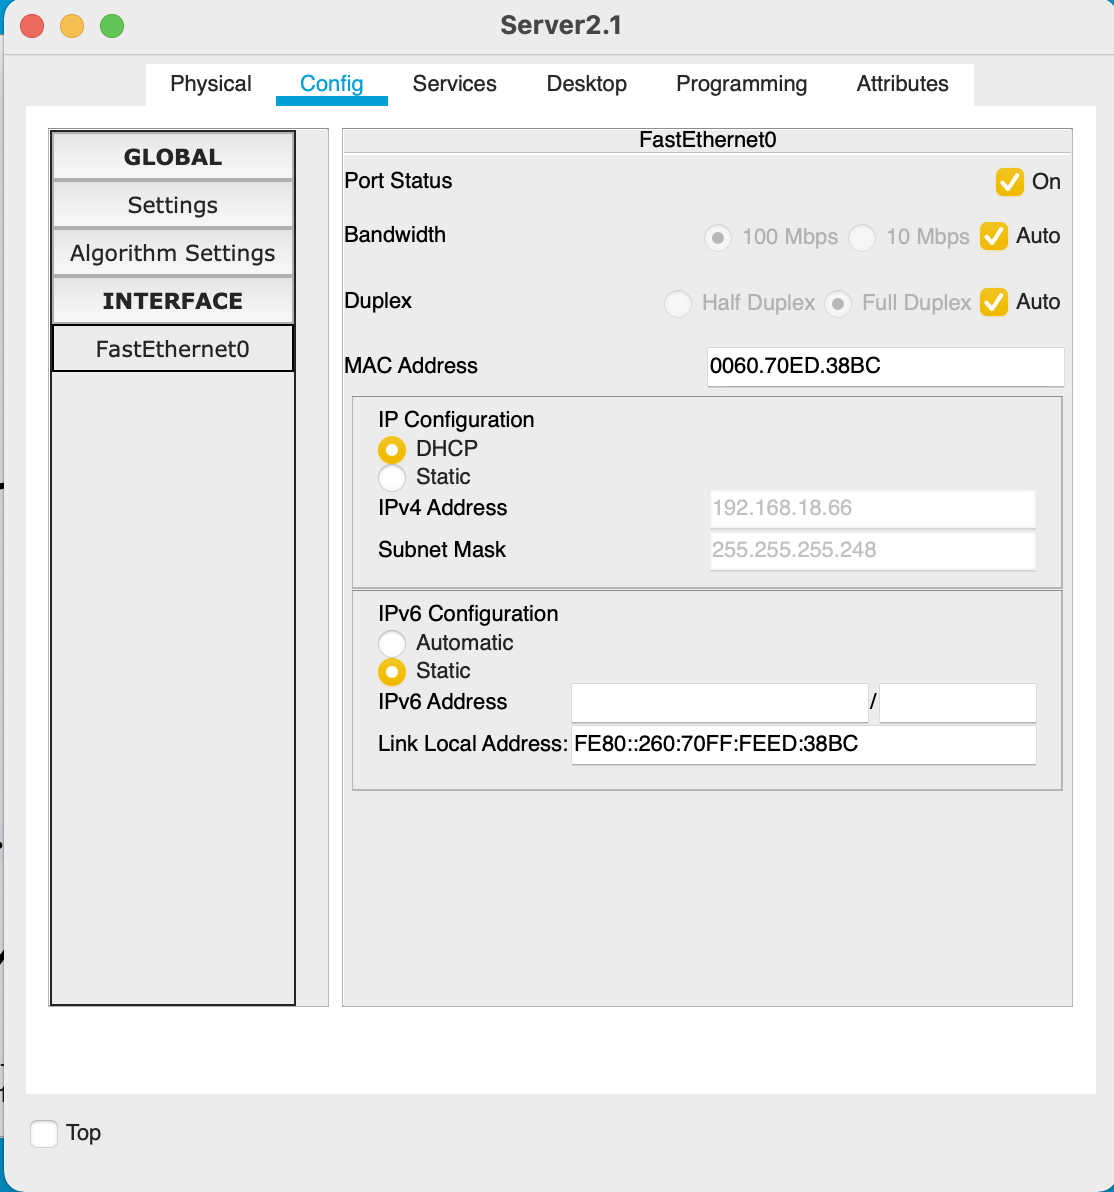
\includegraphics[scale=0.7]{5}
  \caption{Проверка автоматически установленного адреса хоста. }
\end{figure}

\newpage 

\item Настроить в качестве DHCP-сервера маршрутизаторы для подсети 3. 

\begin{figure}[H]\center
	\begin{tabular}{cc}
		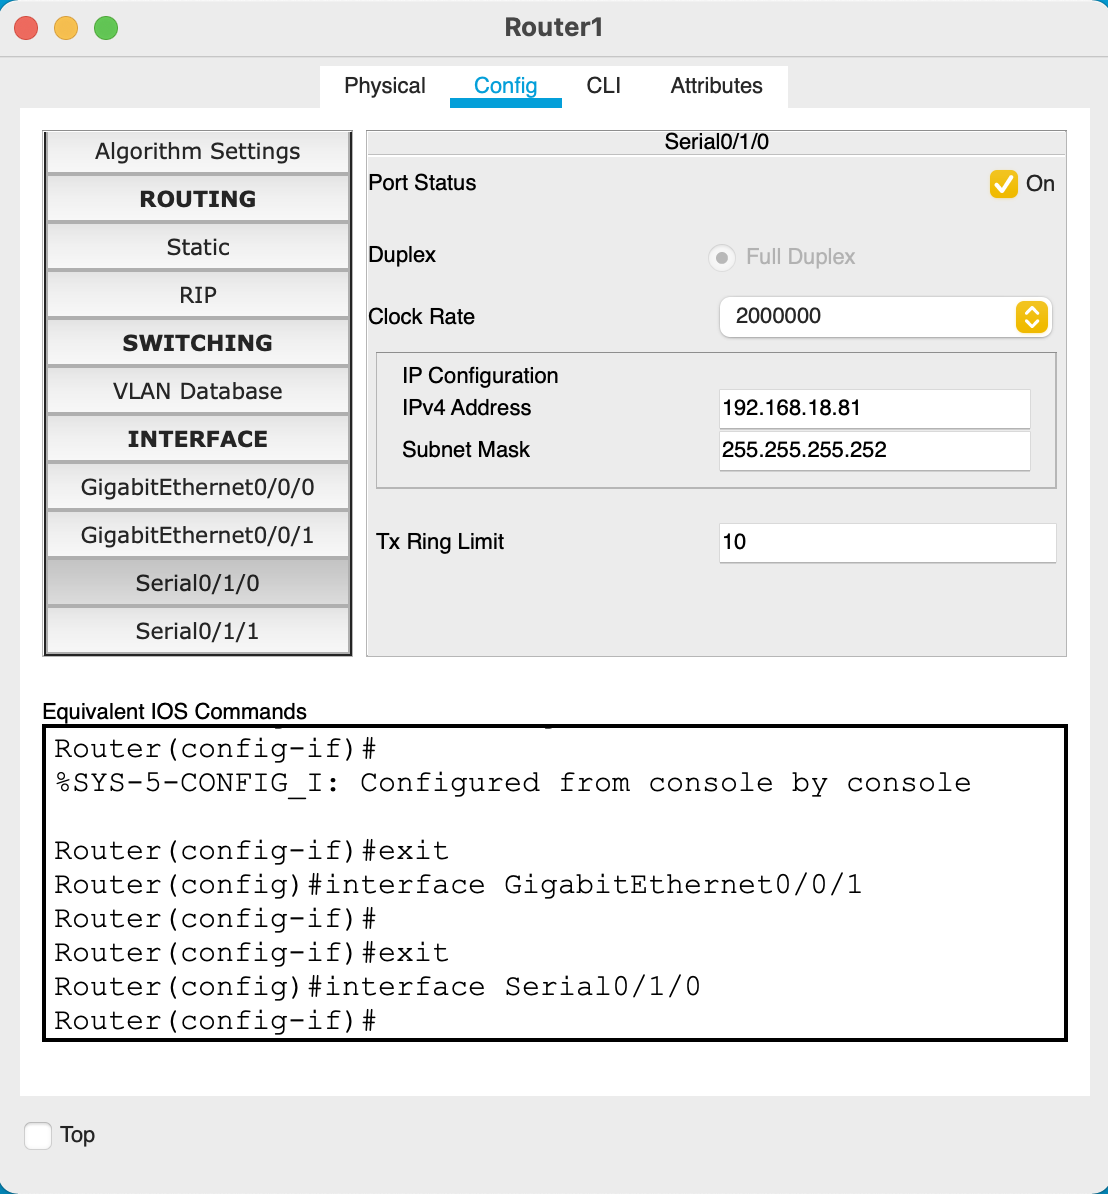
\includegraphics[scale=0.47]{6}&
		 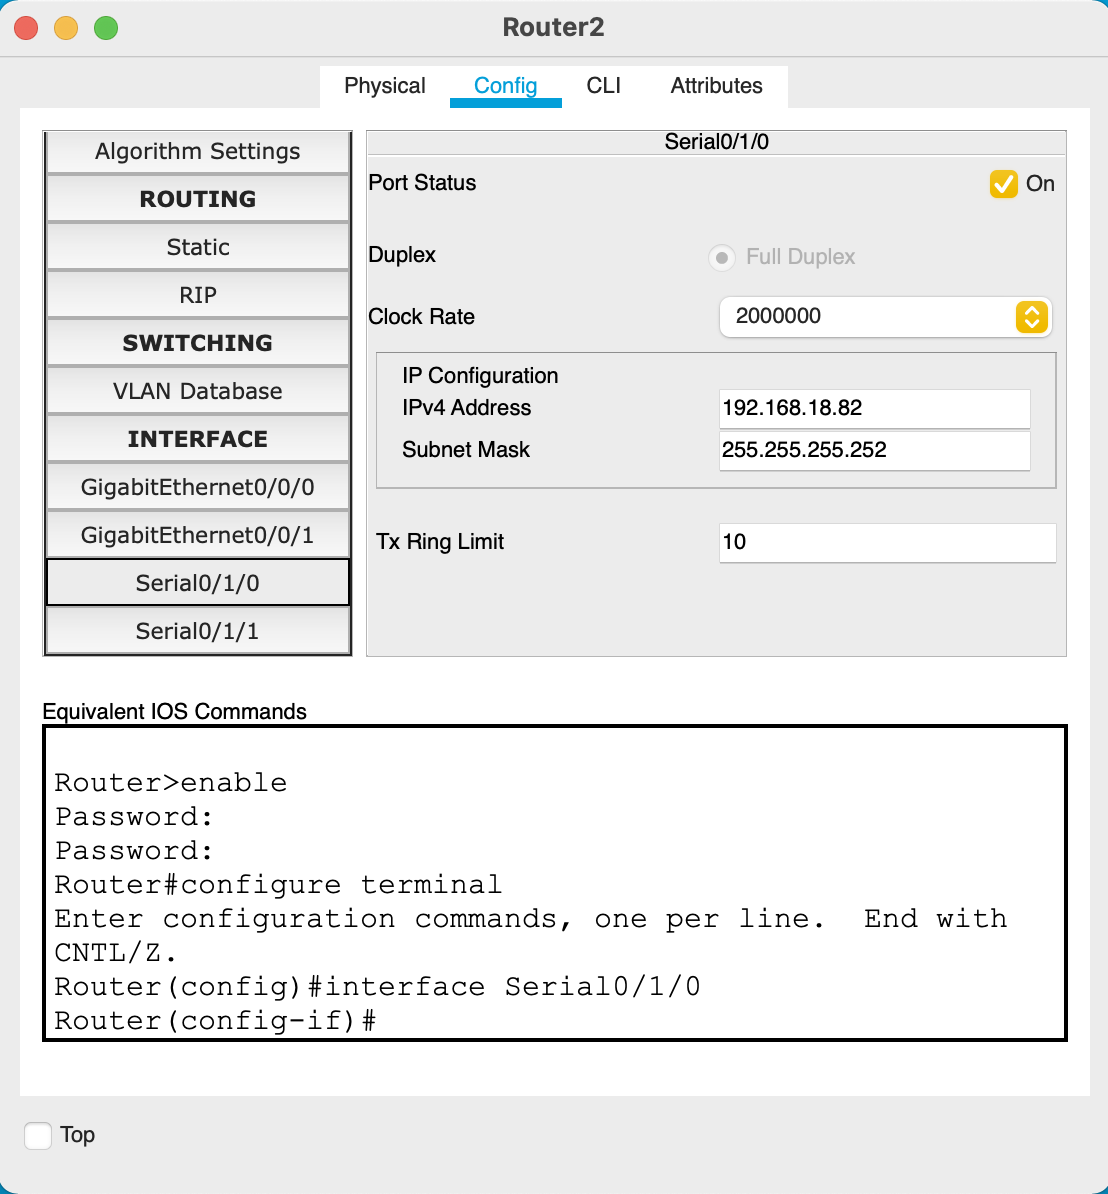
\includegraphics[scale=0.47]{7} \\
	\end{tabular}
	\caption{Настройка маршрутизаторов. }
\end{figure}

\item Схема

\begin{figure}[H]
  \centering
  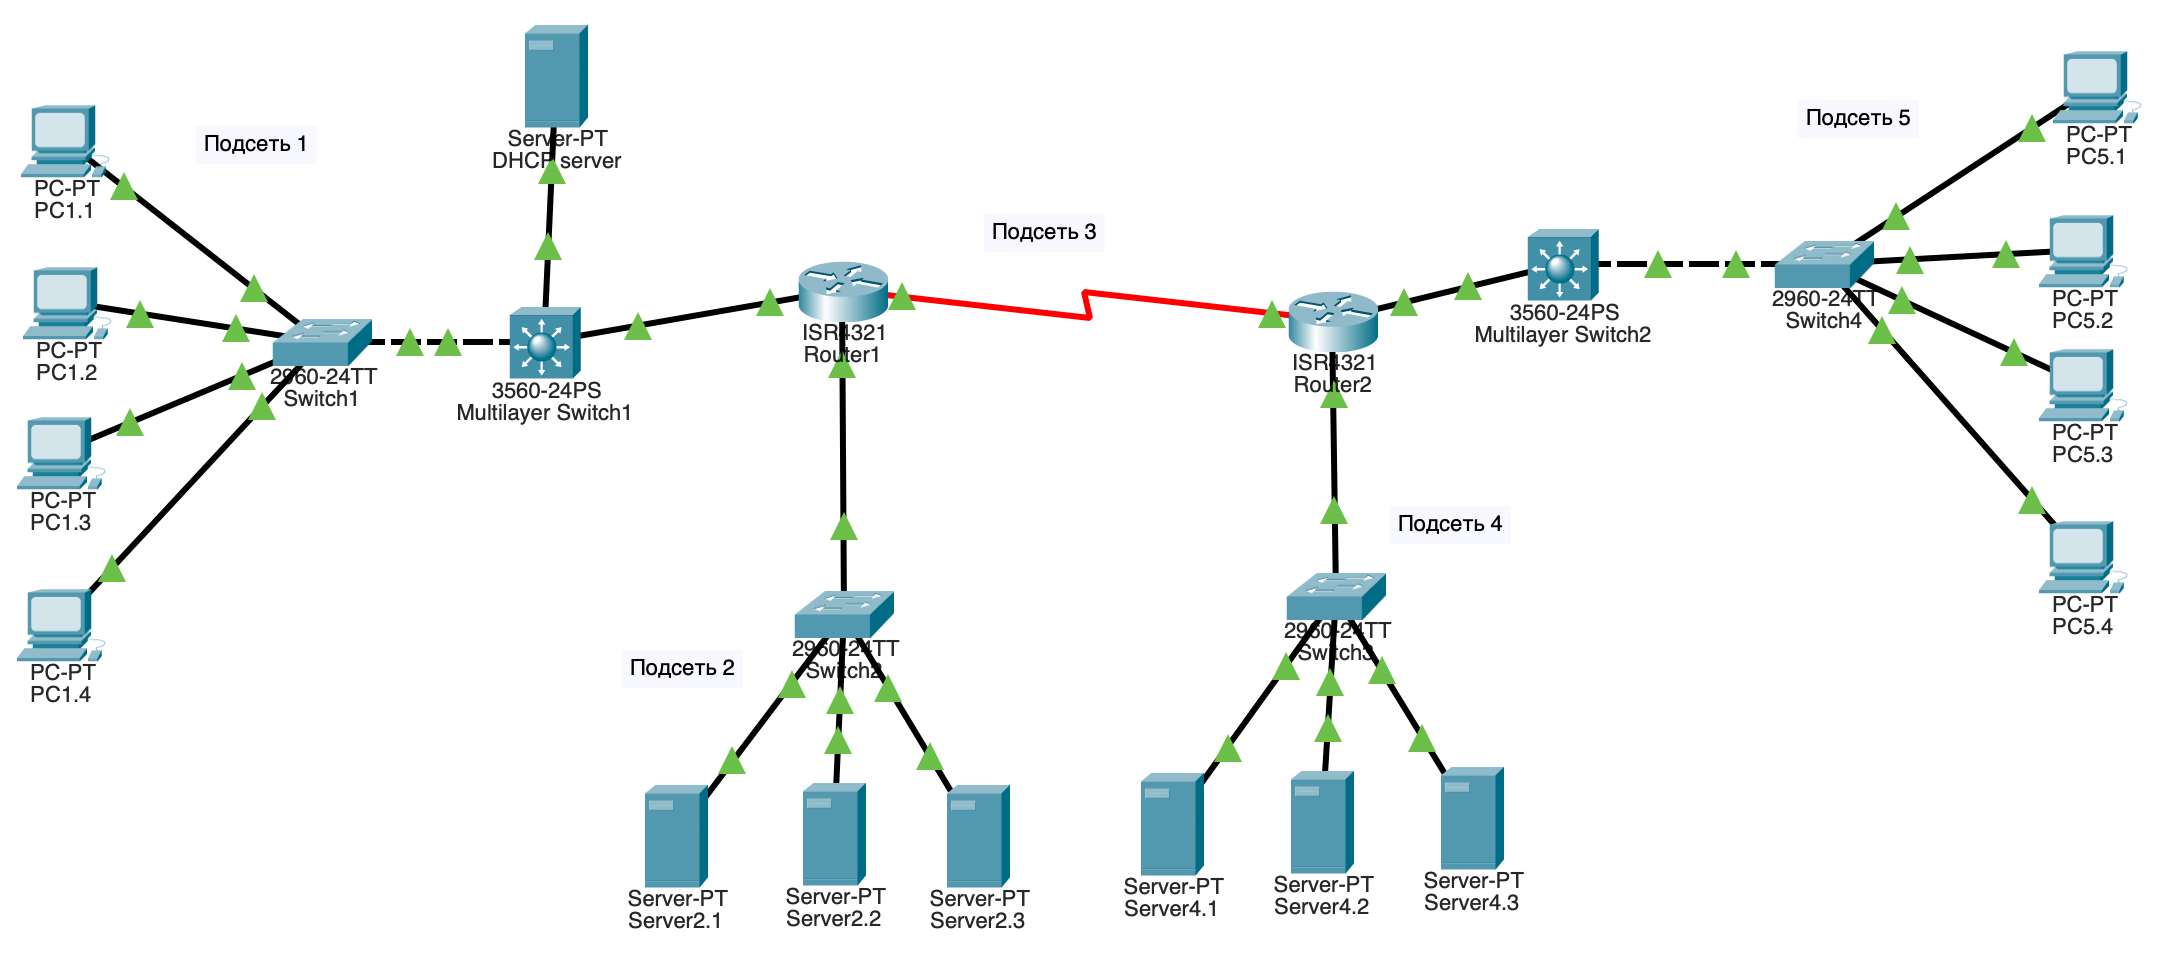
\includegraphics[scale=0.5]{8}
  \caption{Схема. }
\end{figure}

\newpage

\item Проверка работоспособности

Для этого отправим ping на хост в подсети и вне ее (в другую подсеть). 

\begin{figure}[H]
  \centering
  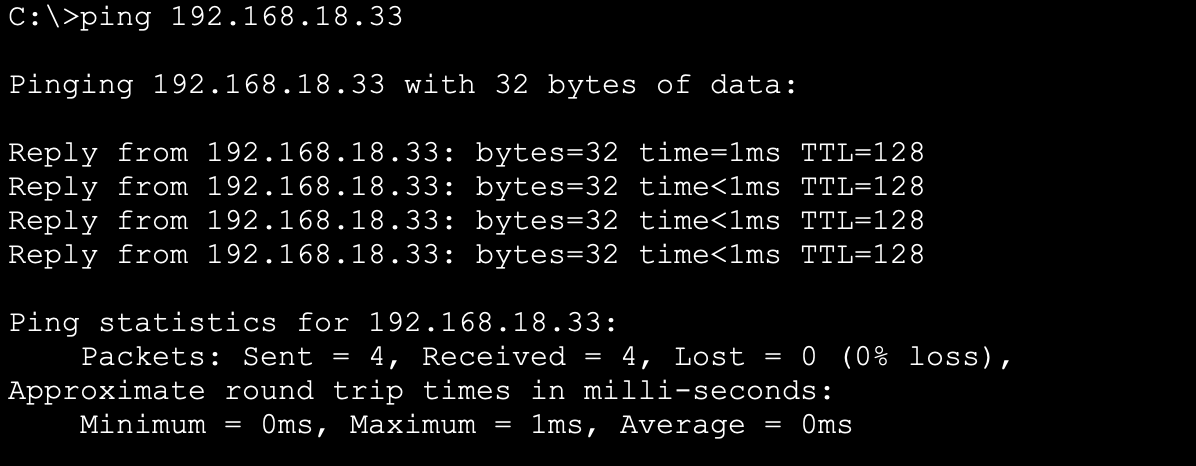
\includegraphics[scale=0.7]{9}
  \caption{Ping в этой подсети. }
\end{figure}

\begin{figure}[H]
  \centering
  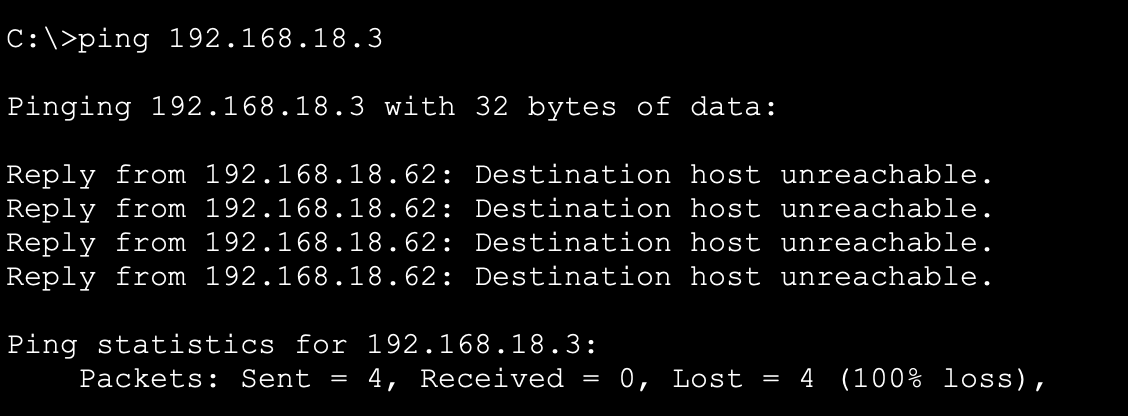
\includegraphics[scale=0.7]{10}
  \caption{Ping в другую подсеть. }
\end{figure}

\end{enumerate}


\end{document}